\section{Data Model Goals}
The schema must make finite-resource correctness enforceable in PostgreSQL,
support short transactions, retain historical monetary values, provide an
auditable booking lifecycle, and serve ownership/operation/expiry queries with
purpose-built indexes.

\section{Core Entities}
Concert/category/inventory tables own the sellable catalog; booking/items own
the reservation and price snapshot. Voucher redemptions, idempotency records,
and status history preserve promotion, retry, and lifecycle evidence. The ERD
is the compact source for table relationships and critical fields.

\section{Entity Relationship Diagram}
Figure~\ref{fig:erd} shows the implemented schema. A transactional
\code{outbox\_events} table is intentionally absent because the outbox remains
an ADR-backed future option rather than submitted runtime behavior.

\clearpage
\begin{landscape}
\begin{figure}[H]
\centering
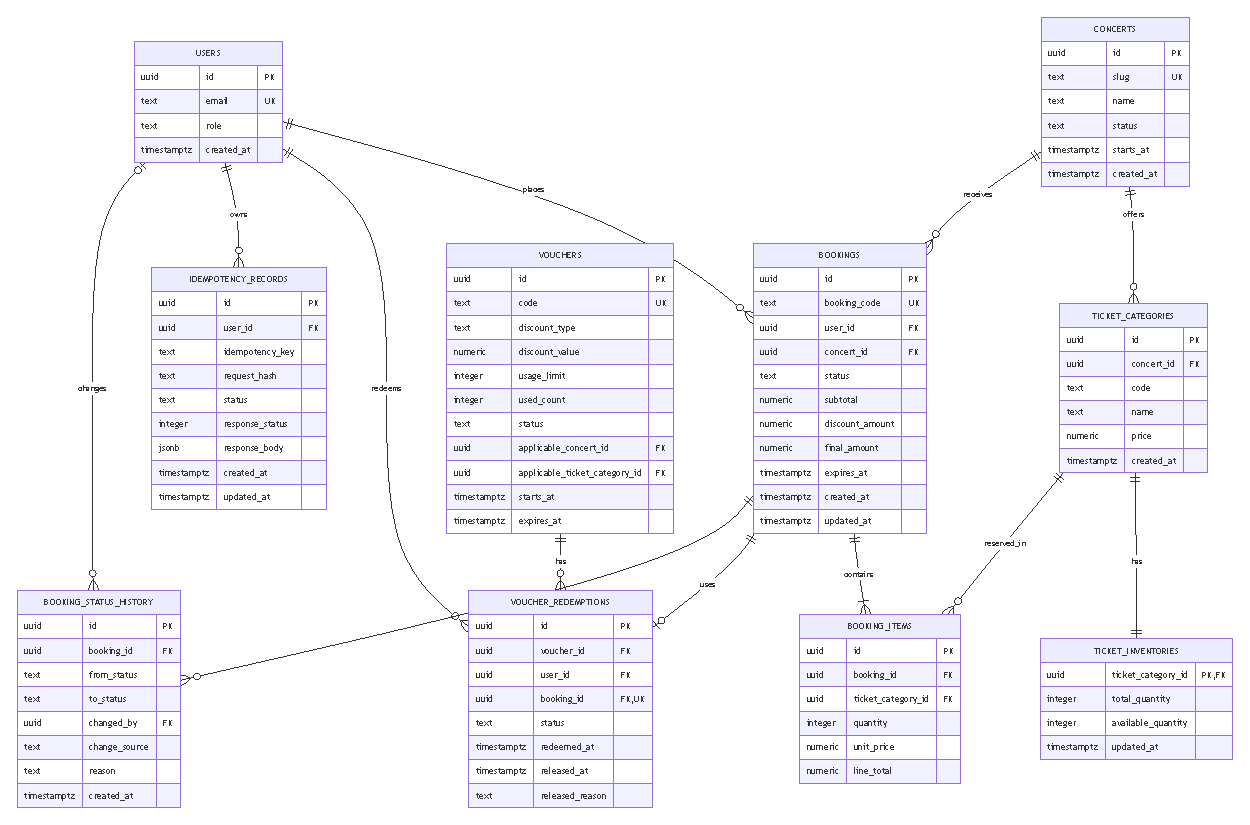
\includegraphics[width=0.98\linewidth,height=0.90\textheight,keepaspectratio]{figures/erd.pdf}
\caption{Implemented PostgreSQL entity relationship model}
\label{fig:erd}
\end{figure}
\end{landscape}
\clearpage

\section{Critical Constraints}
\begin{lstlisting}[language=SQL,caption={Representative database constraints}]
ALTER TABLE ticket_inventories
  ADD CONSTRAINT chk_inventory_non_negative
  CHECK (available_quantity >= 0),
  ADD CONSTRAINT chk_inventory_not_above_total
  CHECK (available_quantity <= total_quantity);

CREATE UNIQUE INDEX uq_idempotency_user_key
  ON idempotency_records(user_id, idempotency_key);

CREATE UNIQUE INDEX uq_voucher_user
  ON voucher_redemptions(voucher_id, user_id)
  WHERE status <> 'RELEASED';
\end{lstlisting}

\section{Index Strategy}
Indexes should follow real query patterns rather than blanket indexing.

\begin{table}[H]
\centering
\caption{Example query-to-index mapping}
\begin{tabularx}{\textwidth}{YY}
\toprule
\textbf{Query Pattern} & \textbf{Suggested Index} \\
\midrule
Expire old reservations & \code{bookings(status, expires\_at)} \\
Customer booking history & \code{bookings(user\_id, created\_at)} \\
Operation filter by concert/status & \code{bookings(concert\_id, status, created\_at)} \\
Voucher lookup by code & unique \code{vouchers(code)} \\
Idempotency replay & unique \code{idempotency\_records(user\_id, idempotency\_key)} \\
\bottomrule
\end{tabularx}
\end{table}

\section{Price Snapshotting}
The request never supplies an authoritative total. The server reads current ticket price and promotion policy, calculates the amount, and persists immutable snapshots in \code{booking\_items} and \code{bookings}. This prevents future catalog changes from rewriting booking history.
